% Content for Chapter 5, Section 5.3 — pulled in by chapters/05-system-design.tex
بُني تطبيق الويب بمكتبة \en{React 19} فوق أداة البناء \en{Vite}، وقُسّم إلى شرائح وظيفية (\en{Feature Slices}) لا إلى طبقات تقنية. وتملك كل شريحة مجلّداتها الأربعة: \en{api} لنداءات الخدمات، و\en{hooks} لحالة الخادم، و\en{components} لعناصر الواجهة، و\en{types} لأنماط البيانات. ويعرض الشكل~\ref{fig:comp-07} هذه المكوّنات مع روابطها الخارجية.

\begin{figure}[htbp]
  \centering
  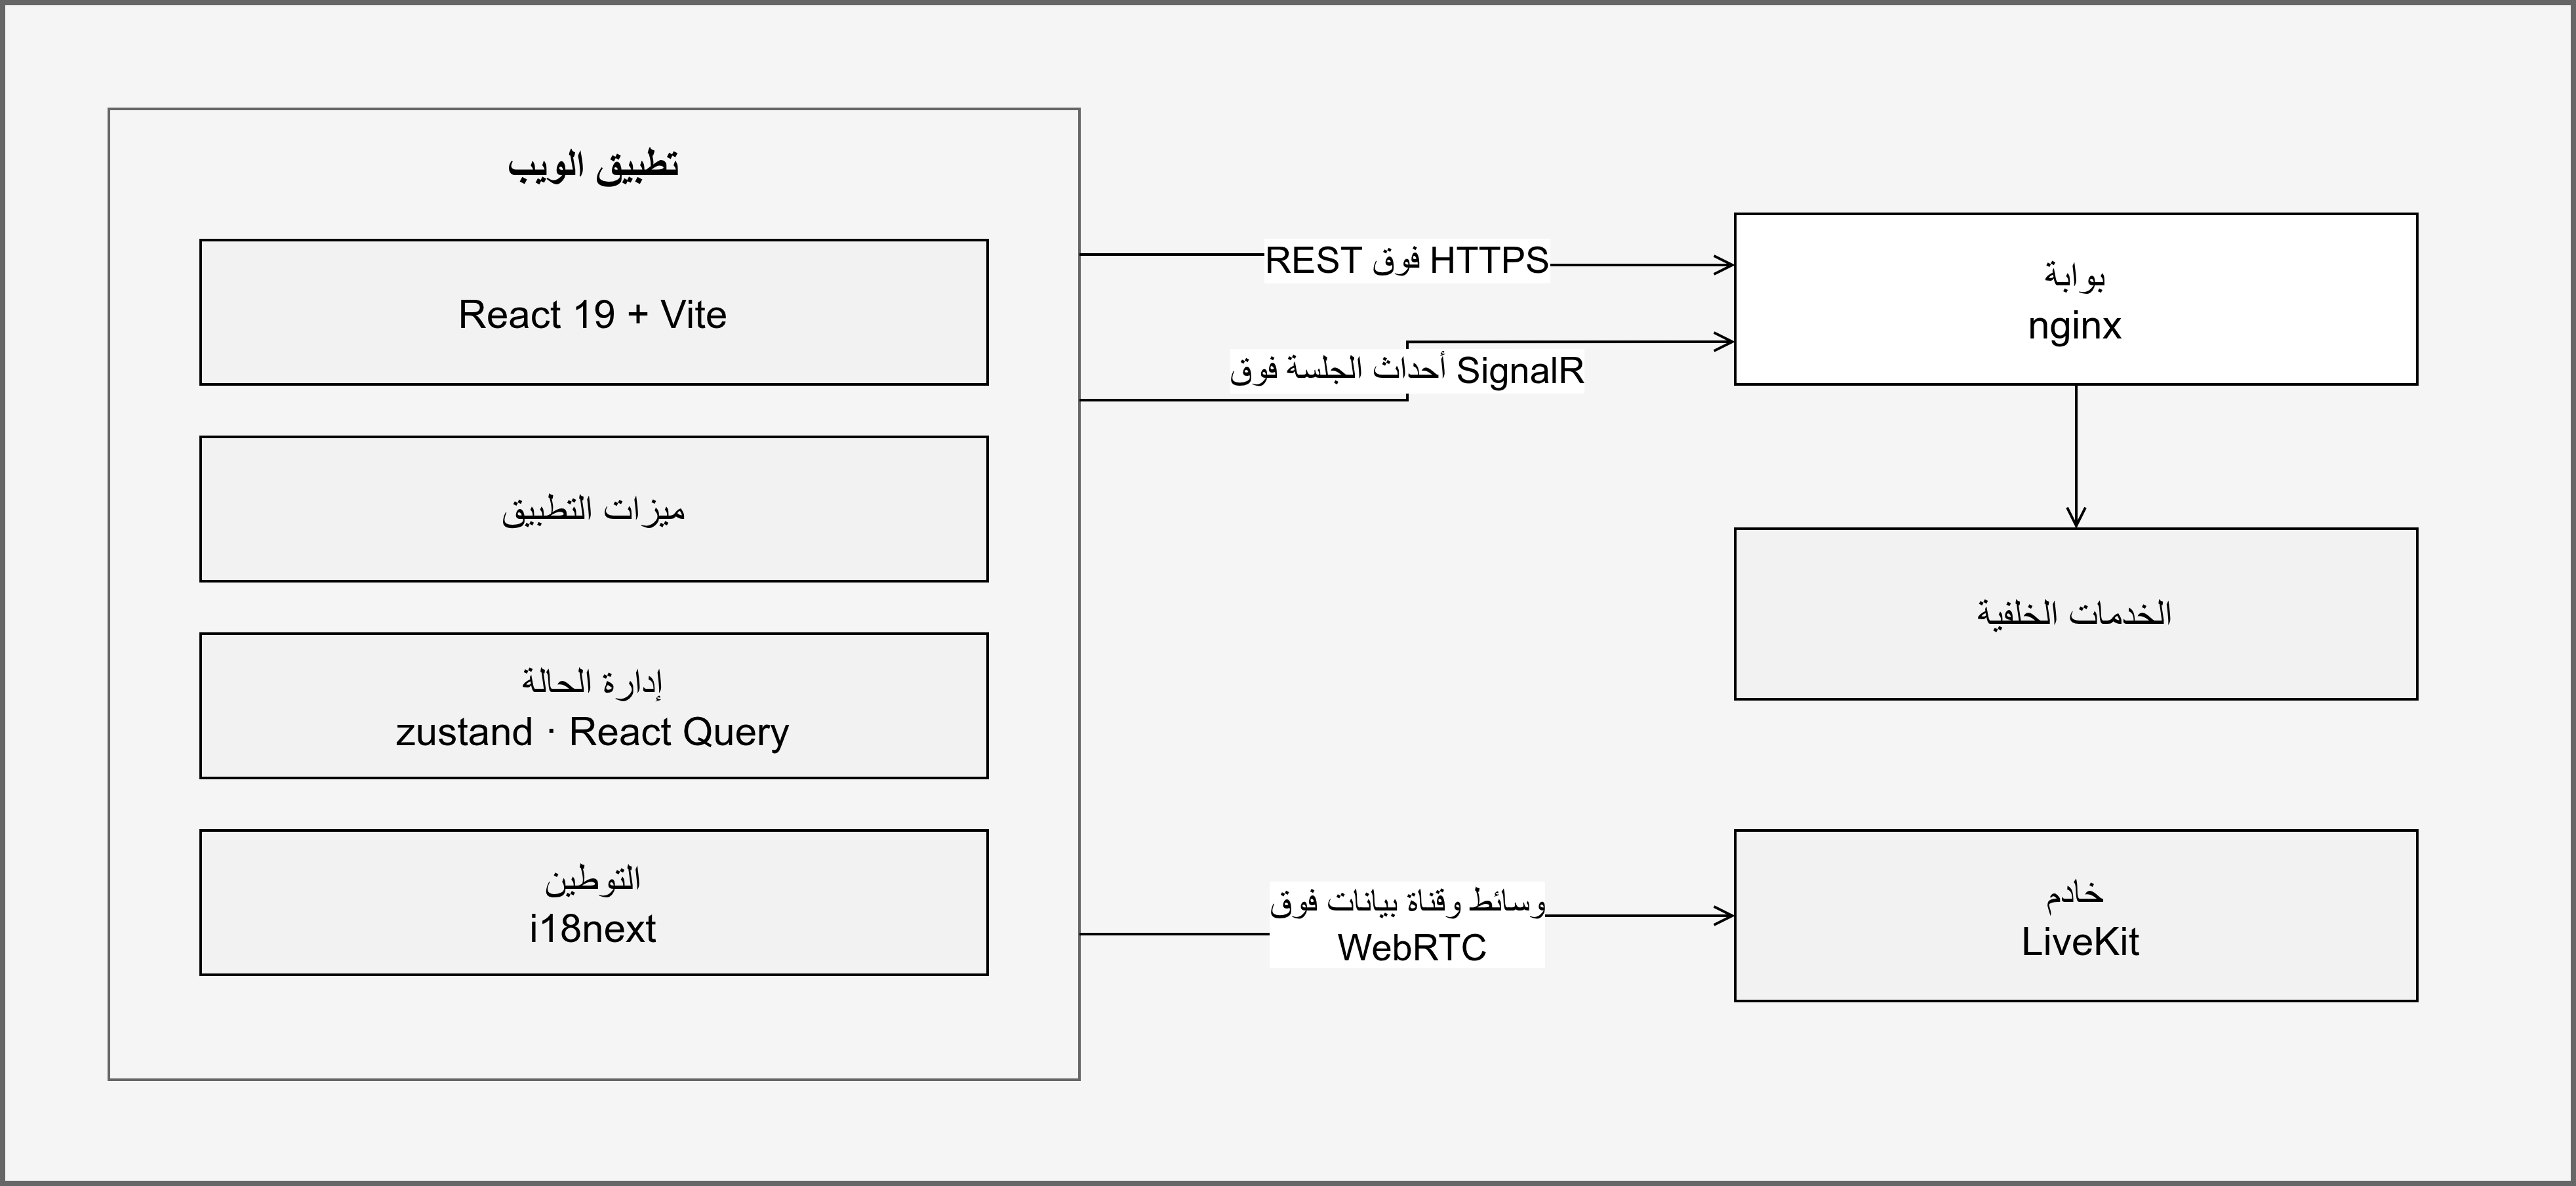
\includegraphics[width=\textwidth,height=0.8\textheight,keepaspectratio]{figures/comp-07-frontend.png}
  \caption{مخطط مكوّنات تطبيق الويب.}
  \label{fig:comp-07}
\end{figure}

ويقوم تصميم التطبيق على أربعة قرارات:

\begin{enumerate}
  \item \textbf{التقسيم بحسب الوظيفة}: تقابل الشرائح الثلاث عشرة مجالاتِ الخدمات الخلفية، فيبقى أثر أيّ تغيير محصورًا في شريحة واحدة. ويقابل التقسيم بحسب الطبقة التقنية ذلك بتوزيع الوظيفة الواحدة على مجلّدات متباعدة.
  \item \textbf{حدّ وحيد للاتصال}: تمرّ نداءات الشرائح كلّها عبر عميل \en{HTTP} واحد هو \en{apiClient}. ويُلحق هذا العميل رمز الوصول بكل طلب، ويعالج الجواب \en{401} بتجديد الرمز وإعادة إرسال الطلب مرّةً واحدة. فإن فشل التجديد محا الجلسة المحلية وأعاد التوجيه إلى صفحة الدخول، دون أن تعلم الشريحة الطالِبة بشيء من ذلك.
  \item \textbf{حراسة على مستوى المسار}: تمنع المكوّنات \en{ProtectedRoute} و\en{PublicRoute} و\en{RoleProtectedRoute} عرض المسارات غير المصرَّح بها للمستخدم الحالي. وهذه الحراسة طبقة إضافية لا حدٌّ أمني، إذ يجري التحقّق الفعلي من الصلاحية في الخدمات الخلفية عند كل طلب.
  \item \textbf{ثلاث قنوات متمايزة}: تُنقَل نداءات \en{REST} وأحداث الجلسة عبر البوّابة العكسية، الأولى فوق \en{HTTPS} والثانية فوق \en{SignalR}. أمّا الوسائط فتُنقَل عبر \en{WebRTC} مباشرةً إلى خادم \en{LiveKit} دون المرور بالبوّابة. وتجري السبّورة التشاركية على قناة بيانات \en{LiveKit} نفسها، فلا تمرّ خطوطها بالخلفية أصلًا.
\end{enumerate}

وتُدار الحالة المشتركة بمخزنَي \en{zustand}: مخزن الجلسة (\en{useAuthStore}) ومخزن السمة (\en{useThemeStore}). وتُدار حالة الخادم في خطّافات كل شريحة بوساطة \en{React Query}. ويدعم التطبيق العربية والإنكليزية عبر \en{i18next} مع تبديل اتجاه الصفحة تبعًا للّغة المختارة.
